\section{Our Chip}
\label{sec:our_setup}

Our device consists of four star-shaped transmon qubits: two storage qubits and two emitter.
All of them are flux-tunable and thus coupled to a flux line.

\begin{figure}[h]
    \centering
    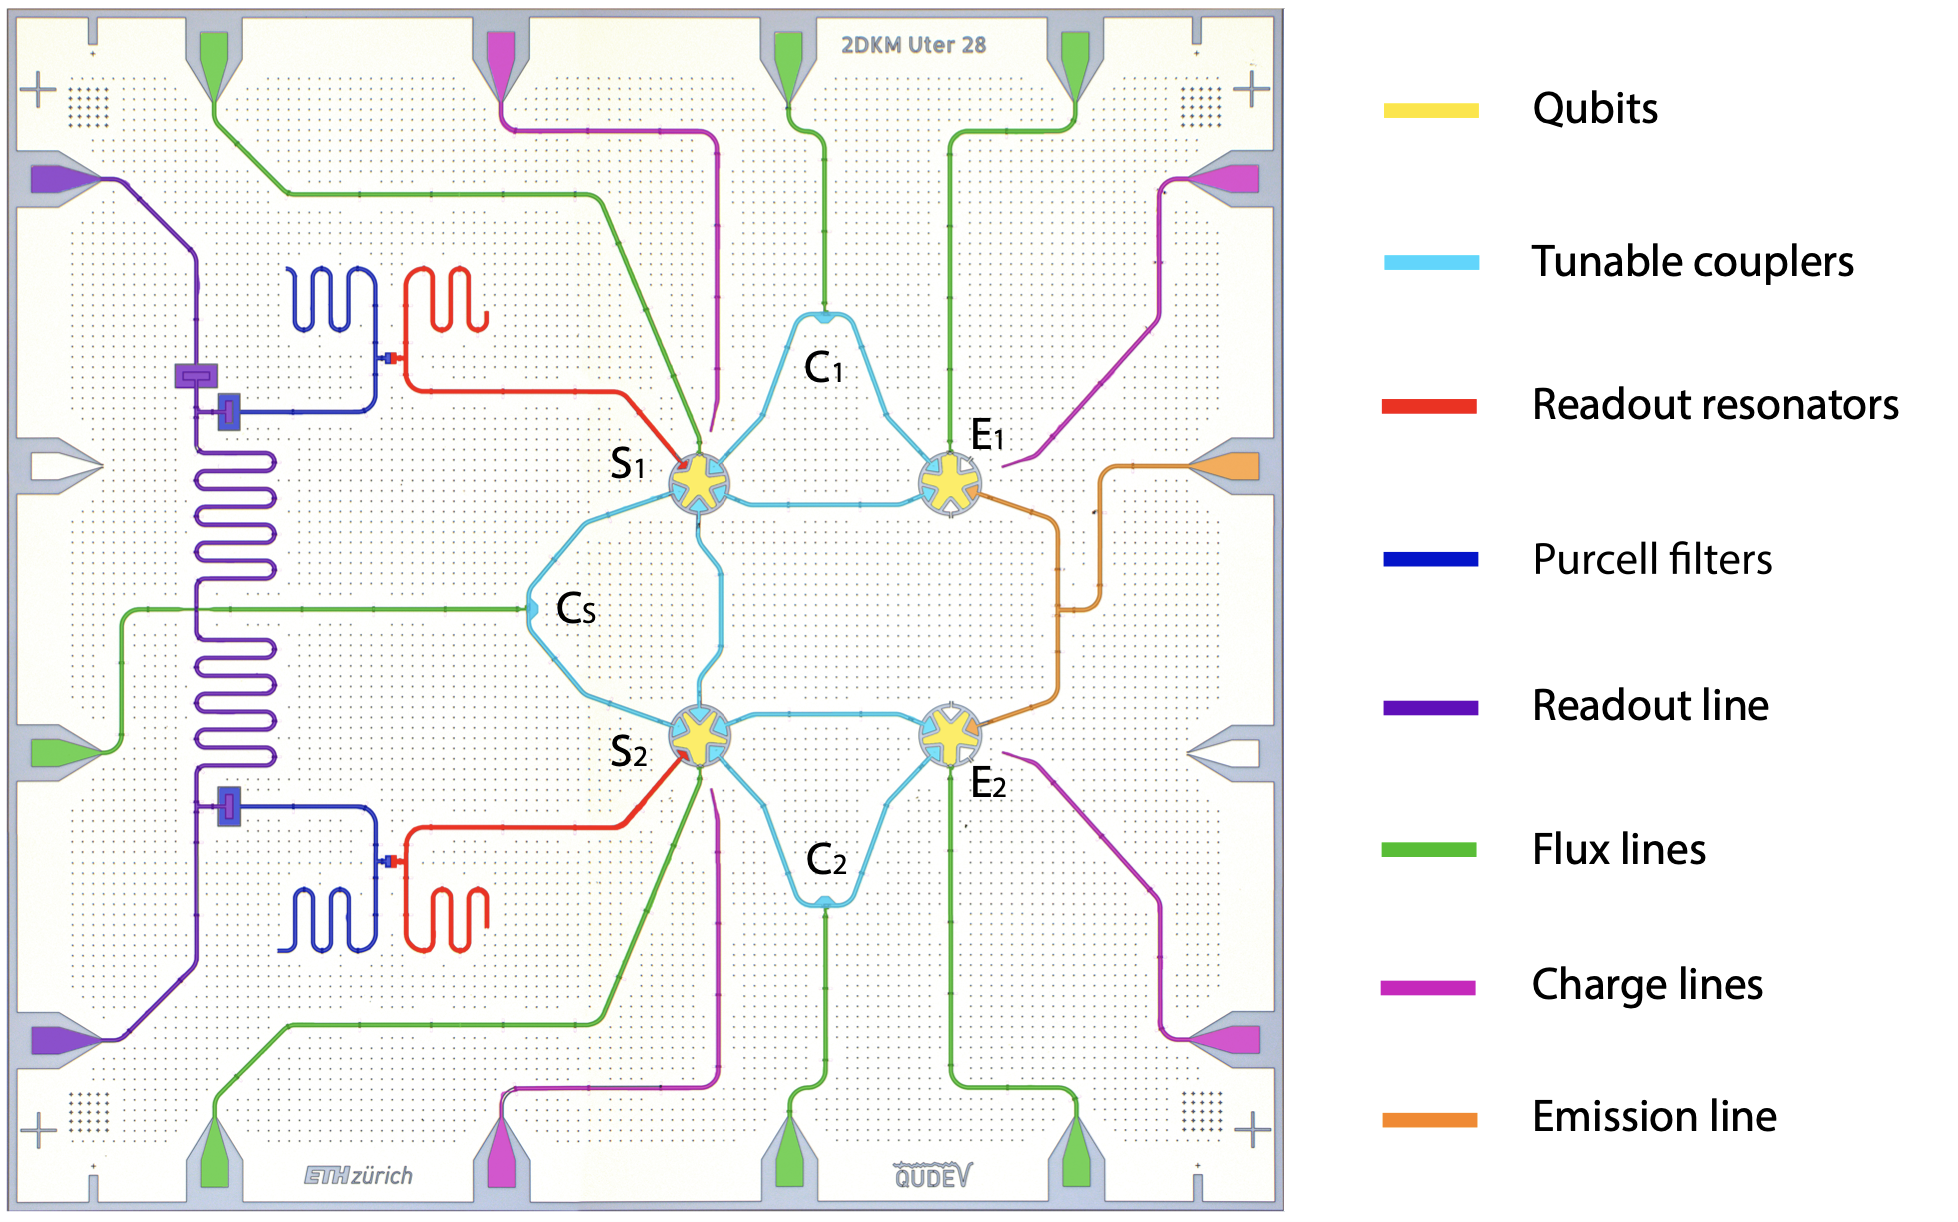
\includegraphics[width = 0.8\textwidth]{Images/Chap1/our_chip.png}
    \caption{False-color micrograph of the employed four-qubit device}
    \label{fig:our_chip}
\end{figure}

\subsection{Storage Qubits}
The storage qubits, depicted with an ‘S' in \cref{fig:our_chip}, are coupled to each other through a tunable coupler ($\text{C}_\text{S}$).
They possess extended lifetimes, enabling us to execute multiple operations on them before their decay or undergo decoherence.
The storage qubits are connected to both a readout resonator and a Purcell filter, utilized for calibration purposes.

\subsection{Emitter Qubits}
Each storage qubit is connected to an emitter qubit, denoted by an ‘E' in the diagram, through tunable couplers ($\text{C}_1$ and $\text{C}_2$).
They are characterized by a very strong coupling to a waveguide referred to as ‘‘emission line''.
This leads to a rapid decay of any excitation induced in them via the emission line, manifesting as emitted photons.
This prevents us from conducting multiple operations on these qubits, since any excitation would be promptly released into the emission line.
Finding a good DC flux for the tunable couplers linking storage and emitter qubits is crucial to avoid the decay of the former into the ladder and subsequently into the environment
